\section{Opposition phases}
An interesting constellation to study the propagation of \acp{ICME} is the so-called opposition, where two planets (or spacecraft) are closely aligned in heliospheric longitude. Near these oppositions, CMEs that are seen in situ at one of these locations are most likely to be seen at the other as well, which allows to investigate their radial evolution.

Some previous studies, such as the model proposed by \citet{Gopalswamy-2001} --- a predecessor of the \acl{DBM}\acused{DBM} (\acs{DBM}, see \autoref{sec:cmes}) --- have stated that the deceleration of fast \acp{CME} due to their interaction with the slower ambient solar wind ceases before \SI{1}{\AU}, e.g. at distances between \SIrange[range-phrase={\,and\,}]{0.75}{0.85}{\AU}. \citet{Winslow-2015} have validated this hypothesis using measurements at Mercury and \citet{Wang-2005} have shown measurements from the \textit{Ulysses} spacecraft, mostly far beyond \SI{1}{\AU}, that show no significant deceleration. However, observations at Mars, which  is located at a heliocentric distance of $\sim\SI{1.5}{\AU}$ have not been included in such investigations so far.

In the case of Earth and Mars, whose orbital periods are 365 and 687 days, respectively, an opposition occurs approximately every 2.1 years. Since the \textit{Curiosity} rover's landing on Mars in August 2012, there were four such oppositions: In April 2014, May 2016, July 2018, and October 2020. The following study will present the first statistical study of \acp{ICME} and the associated \acp{FD} during the first two of these opposition periods, and during oppositions of Mars with one of the two \ac{STEREO} spacecraft in 2012 and 2013. The \acp{FD} were detected at the two locations using the \acl{MSL}\acused{MSL} \acl{RAD}\acused{RAD} (\acp{MSL}/\acp{RAD}, \autoref{sec:mslrad}), the South Pole neutron monitor at Earth (\autoref{sec:neutronmonitors}) and the \ac{STEREO} \ac{HET}. These datasets were then used to derive the \ac{ICME} propagation time between \SI{1}{\AU} and Mars. In the study, we compare the derived transit speed between \SI{1}{\AU} and Mars to the in situ measured velocity at \SI{1}{\AU} as well as the launch speed at the Sun to show that fast \acp{ICME} still decelerate beyond \SI{1}{\AU}. Comparisons with the WSA-ENLIL+Cone and \ac{DBM} models are also performed to investigate their accuracy for predicting \ac{ICME} arrival times at Mars.

The following article is reproduced from \textcite{Forstner-2018} with permission from Journal of Geophysical Research: Space Physics, \copyright American Geophysical Union:\\

\noindent\pubcite{Forstner-2018}\\
\strut\hfill Own contribution: 90\%

\newpage
\newcounter{includepdfpageJGREighteen}

\addtocounter{subsection}{1}
\setcounter{subsubsection}{1} 
\phantomsection
\addcontentsline{toc}{subsection}{\arabic{chapter}.\arabic{section}.\arabic{subsection} Using Forbush Decreases to Derive the Transit Time of ICMEs Propagating from 1 AU to Mars (Publication JGR--Space Physics 2018)}
%
\phantomsection
\addcontentsline{toc}{subsubsection}{\arabic{chapter}.\arabic{section}.\arabic{subsection}.\arabic{subsubsection} Introduction}
\label{sec:paper_forstner2018}
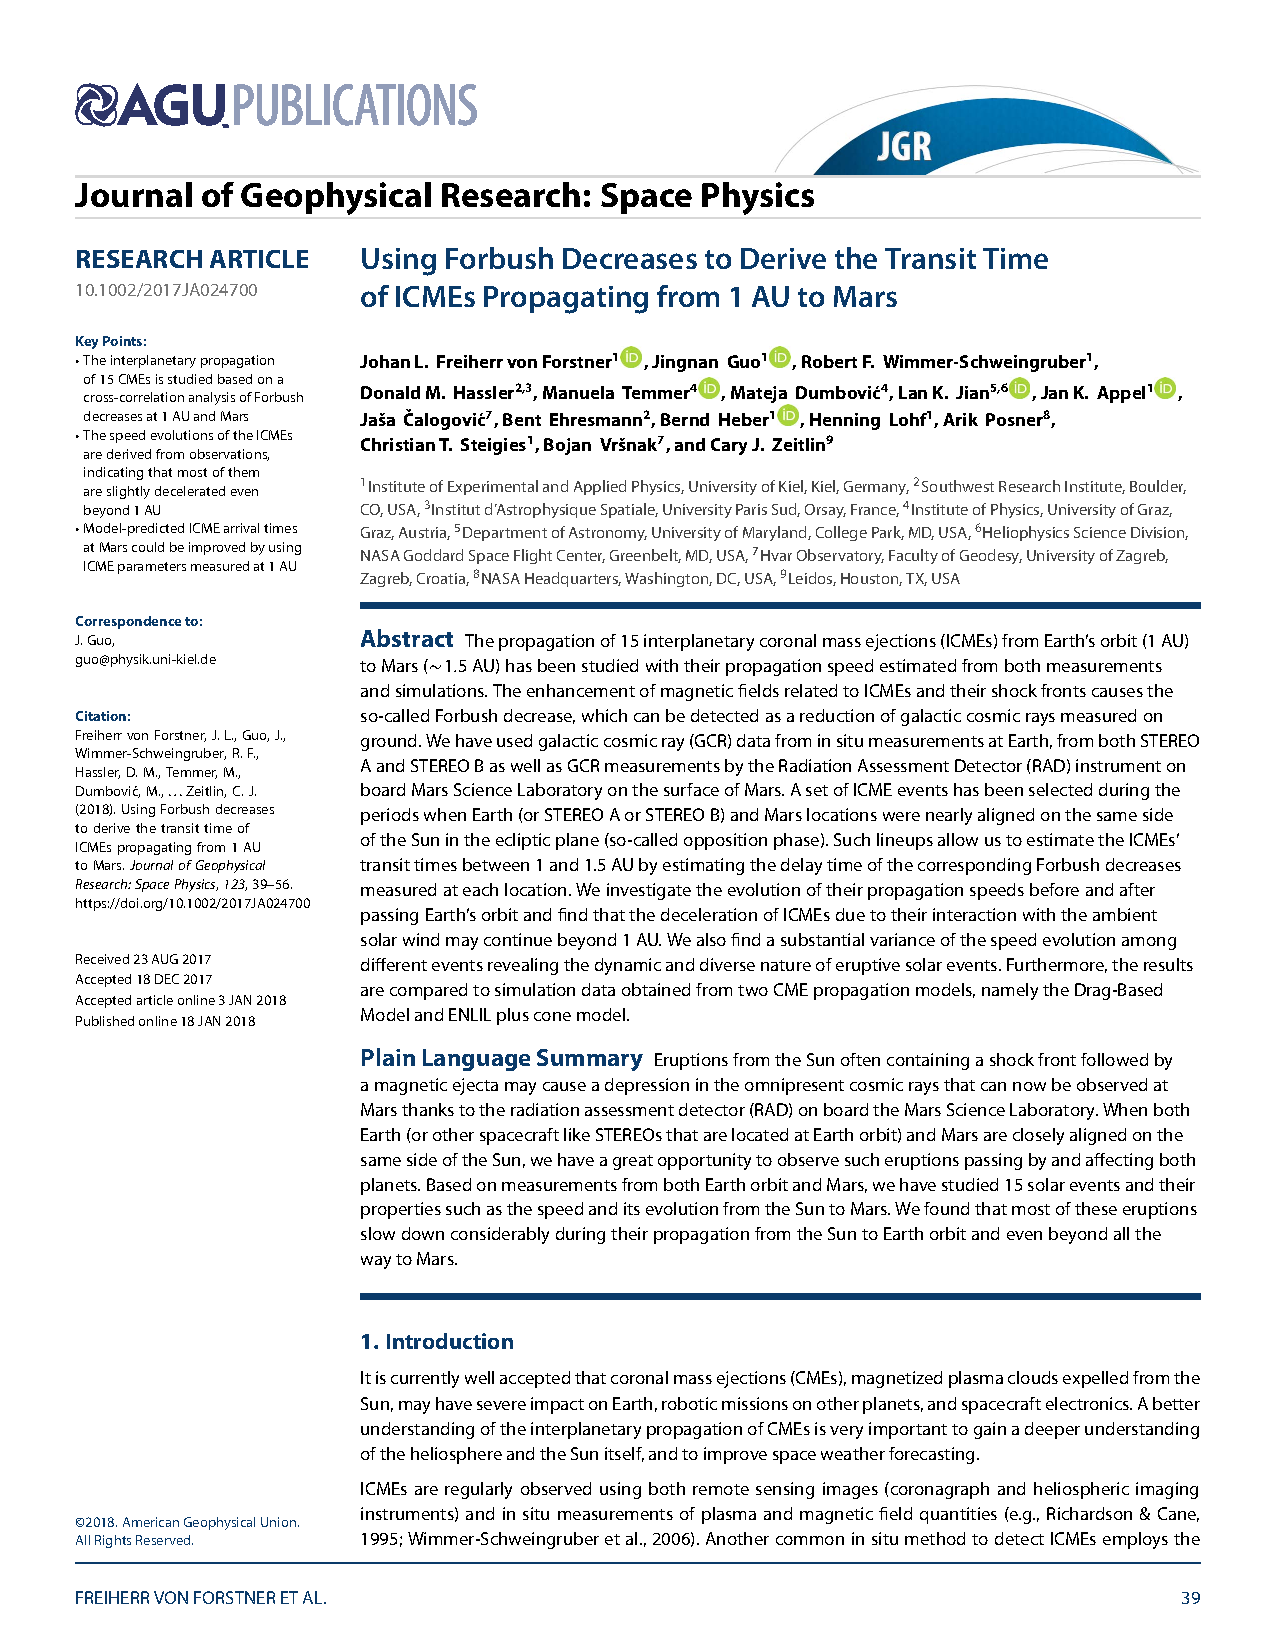
\includepdf[pages={1-2}, link, linkname=paper_forstner2018, scale=.9, pagecommand={\refstepcounter{includepdfpageJGREighteen}\label{paper_forstner2018.\theincludepdfpageJGREighteen}}]{publications/Forstner_et_al-2018-JGRSpace.pdf}
%
\addtocounter{subsubsection}{1} 
\phantomsection
\addcontentsline{toc}{subsubsection}{\arabic{chapter}.\arabic{section}.\arabic{subsection}.\arabic{subsubsection} Methods and Data}
\includepdf[pages={3-5}, link, linkname=paper_forstner2018, scale=.9, pagecommand={\refstepcounter{includepdfpageJGREighteen}\label{paper_forstner2018.\theincludepdfpageJGREighteen}}]{publications/Forstner_et_al-2018-JGRSpace.pdf}
%
\addtocounter{subsubsection}{1} 
\phantomsection
\addcontentsline{toc}{subsubsection}{\arabic{chapter}.\arabic{section}.\arabic{subsection}.\arabic{subsubsection} Results and Discussion}
\includepdf[pages={6-12}, link, linkname=paper_forstner2018, scale=.9, pagecommand={\refstepcounter{includepdfpageJGREighteen}\label{paper_forstner2018.\theincludepdfpageJGREighteen}}]{publications/Forstner_et_al-2018-JGRSpace.pdf}
%
\addtocounter{subsubsection}{1} 
\phantomsection
\addcontentsline{toc}{subsubsection}{\arabic{chapter}.\arabic{section}.\arabic{subsection}.\arabic{subsubsection} Conclusion}
\includepdf[pages={13}, link, linkname=paper_forstner2018, scale=.9, pagecommand={\refstepcounter{includepdfpageJGREighteen}\label{paper_forstner2018.\theincludepdfpageJGREighteen}}]{publications/Forstner_et_al-2018-JGRSpace.pdf}
%
\addtocounter{subsubsection}{1} 
\phantomsection
\addcontentsline{toc}{subsubsection}{\arabic{chapter}.\arabic{section}.\arabic{subsection}.\arabic{subsubsection} Appendix A: Cross-Correlation Analysis Plots for Each Event}
\includepdf[pages={14-16}, link, linkname=paper_forstner2018, scale=.9, pagecommand={\refstepcounter{includepdfpageJGREighteen}\label{paper_forstner2018.\theincludepdfpageJGREighteen}}]{publications/Forstner_et_al-2018-JGRSpace.pdf}
%
\addtocounter{subsubsection}{1} 
\phantomsection
\addcontentsline{toc}{subsubsection}{\arabic{chapter}.\arabic{section}.\arabic{subsection}.\arabic{subsubsection} References}
\includepdf[pages={17-18}, link, linkname=paper_forstner2018, scale=.9, pagecommand={\refstepcounter{includepdfpageJGREighteen}\label{paper_forstner2018.\theincludepdfpageJGREighteen}}]{publications/Forstner_et_al-2018-JGRSpace.pdf}

\section{Heliospheric imager observations}
In the following study, we investigate a separate sample of \acp{ICME} that were detected by the \ac{STEREO} \acp{HI} and propagated towards Mars, validating their arrival times using the \acp{FD} detected at \ac{MSL}/\ac{RAD}. A similar study has been performed by \citet{Moestl-2017-HelcatsHSO} with in situ measurements at different locations in the inner heliosphere, but this is the first validation of Mars arrival times calculated with the \ac{STEREO}-\ac{HI} data. The study also includes some \acp{ICME} that hit the \ac{MSL} spacecraft during its cruise phase.
For the analysis of the HI data, three different single-spacecraft geometric reconstruction methods will be described (fixed $\phi$, harmonic mean, and self-similar expansion), and applied to the J-maps. For an introduction into these methods, see \autoref{sec:stereohi} and references therein.

The results show that the performance of the single-spacecraft fitting methods applied to \ac{HI} data for predicting \acp{ICME} arrivals (see also \autoref{sec:stereohi}) is not flawless, as especially the reconstructed propagation longitude has a large uncertainty: Only \SI{39+-6}{\percent} of the events predicted to hit Mars (or \ac{MSL}) were actually observed with a clear \ac{FD}. This may in part also be due to weak \acp{ICME} or flank encounters, which may not cause a strong \ac{FD}. Still, this value is consistent with the performance scores calculated by \citet{Moestl-2017-HelcatsHSO} for the arrival at other locations closer to the Sun.

At the time of this study, we used version 5 of the \acs{HELCATS} CME kinematics catalog (HIGeoCat), which was updated until the end of September 2017. We have made the arrival time calculations ourselves based on the data available in the HIGeoCat as the arrival time catalog (ARRCAT) had only been updated until September 2014.
After the publication of this study, some updates to the catalog have been released\footnote{\url{https://www.helcats-fp7.eu/catalogues/wp3_cat.html}}, with the latest version from October 8, 2020 containing 82 additional \acp{ICME} (\num{1541} events compared to \num{1459}), which were all observed by \ac{STEREO}-A \ac{HI} as there is still no new data available from \ac{STEREO}-B (see \autoref{sec:stereohi}). According to the arrival time catalog (ARRCAT), which is calculated from these data and has been updated until the end of August 2020 on the \textit{Helio4Cast} website\footnote{\url{https://helioforecast.space/arrcat}}, 13 additional \acp{ICME} detected in the recent years have also been determined to hit Mars based on the \ac{HI} data (5 in 2018, 1 in 2019, and 7 in 2020). The presence of corresponding \ac{MSL}/\ac{RAD} \ac{FD} signatures for these events should be reviewed in future studies.

The following article is reproduced from \textcite{Forstner-2019} with permission from Space 
Weather, \copyright American Geophysical Union:\\

\noindent\pubcite{Forstner-2019}\\
\strut\hfill Own contribution: 90\%

\newpage
\newcounter{includepdfpageSWNineteen}

\addtocounter{subsection}{1}
\setcounter{subsubsection}{1} 
\phantomsection
\addcontentsline{toc}{subsection}{\arabic{chapter}.\arabic{section}.\arabic{subsection} Tracking and Validating ICMEs Propagating Toward Mars Using STEREO Heliospheric Imagers Combined With Forbush Decreases Detected by MSL/RAD (Publication Space Weather 2019)}
%
\phantomsection
\addcontentsline{toc}{subsubsection}{\arabic{chapter}.\arabic{section}.\arabic{subsection}.\arabic{subsubsection} Introduction}
\label{sec:paper_forstner2019}
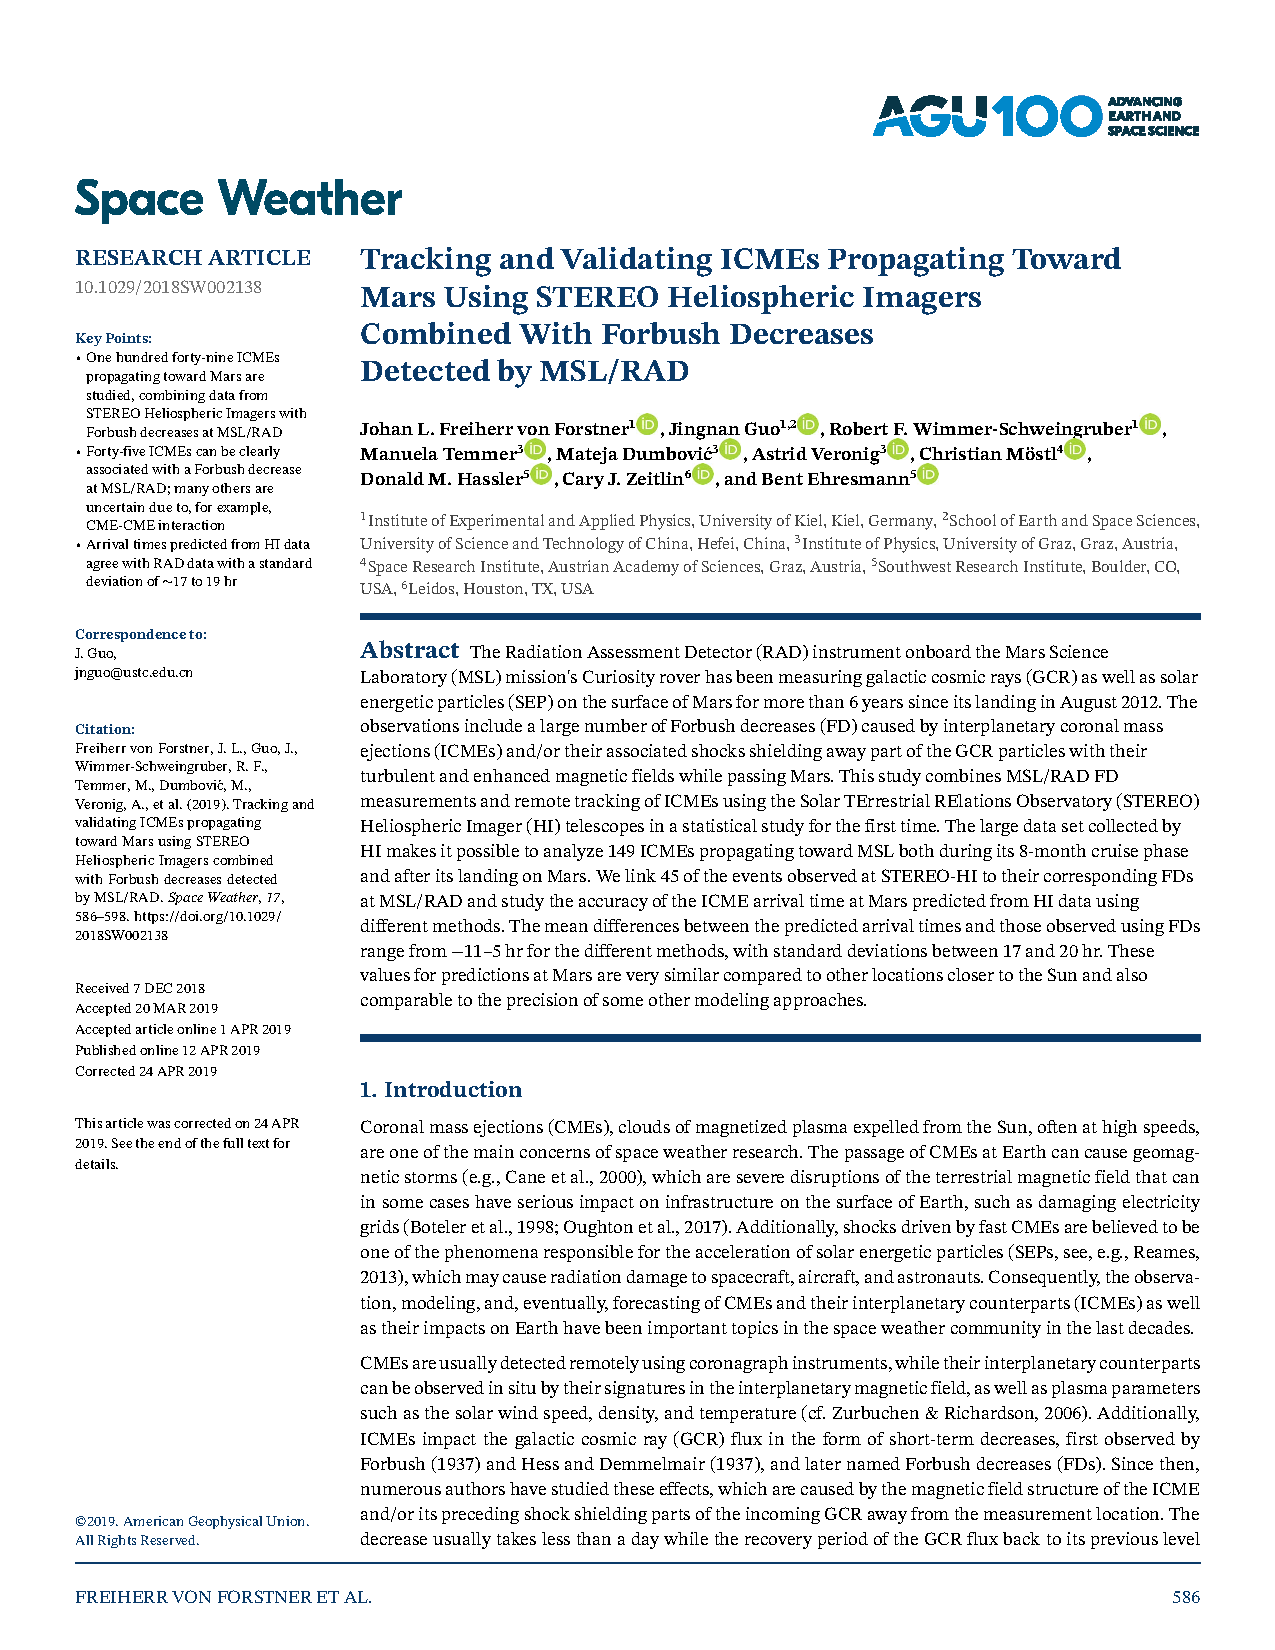
\includepdf[pages={1}, link, linkname=paper_forstner2019, scale=.95, pagecommand={\refstepcounter{includepdfpageSWNineteen}\label{paper_forstner2019.\theincludepdfpageSWNineteen}}]{publications/Forstner_et_al-2019-Space_Weather.pdf}
%
\addtocounter{subsubsection}{1} 
\phantomsection
\addcontentsline{toc}{subsubsection}{\arabic{chapter}.\arabic{section}.\arabic{subsection}.\arabic{subsubsection} Data and Methods}
\includepdf[pages={2-3}, link, linkname=paper_forstner2019, scale=.95, pagecommand={\refstepcounter{includepdfpageSWNineteen}\label{paper_forstner2019.\theincludepdfpageSWNineteen}}]{publications/Forstner_et_al-2019-Space_Weather.pdf}
%
\addtocounter{subsubsection}{1} 
\phantomsection
\addcontentsline{toc}{subsubsection}{\arabic{chapter}.\arabic{section}.\arabic{subsection}.\arabic{subsubsection} Results and Discussion}
\includepdf[pages={4-9}, link, linkname=paper_forstner2019, scale=.95, pagecommand={\refstepcounter{includepdfpageSWNineteen}\label{paper_forstner2019.\theincludepdfpageSWNineteen}}]{publications/Forstner_et_al-2019-Space_Weather.pdf}
%
\addtocounter{subsubsection}{1} 
\phantomsection
\addcontentsline{toc}{subsubsection}{\arabic{chapter}.\arabic{section}.\arabic{subsection}.\arabic{subsubsection} Conclusions and Outlook}
\includepdf[pages={10}, link, linkname=paper_forstner2019, scale=.95, pagecommand={\refstepcounter{includepdfpageSWNineteen}\label{paper_forstner2019.\theincludepdfpageSWNineteen}}]{publications/Forstner_et_al-2019-Space_Weather.pdf}
%
\addtocounter{subsubsection}{1} 
\phantomsection
\addcontentsline{toc}{subsubsection}{\arabic{chapter}.\arabic{section}.\arabic{subsection}.\arabic{subsubsection} References}
\includepdf[pages={11-13}, link, linkname=paper_forstner2019, scale=.95, pagecommand={\refstepcounter{includepdfpageSWNineteen}\label{paper_forstner2019.\theincludepdfpageSWNineteen}}]{publications/Forstner_et_al-2019-Space_Weather.pdf}